\documentclass{standalone}
% This file was created with tikzplotlib v0.9.15.

\usepackage{siunitx}
\usepackage{pgfplots}
% and optionally (as of Pgfplots 1.3):
\pgfplotsset{compat=newest}
\pgfplotsset{plot coordinates/math parser=false}
\newlength\figureheight
\newlength\figurewidth

\newcommand{\Set}[1]{\mathcal{#1}}
\newcommand{\Vector}[1]{\bm{\MakeLowercase{#1}}}
\newcommand{\Operator}[1]{\bm{\MakeUppercase{#1}}}
%%%%%%%%%%
\DeclareMathAlphabet{\mathsfbr}{OT1}{cmss}{m}{n}%for math sans serif (cmss)
\SetMathAlphabet{\mathsfbr}{bold}{OT1}{cmss}{bx}{n}%for math sans serif (cmss)
\DeclareRobustCommand{\msf}[1]{%
  \ifcat\noexpand#1\relax\msfgreek{#1}\else\mathsfbr{#1}\fi%for math sans serif (cmss)
}
\DeclareFontEncoding{LGR}{}{} % or load \usepackage{textgreek}
\DeclareSymbolFont{sfgreek}{LGR}{cmss}{m}{n}
\SetSymbolFont{sfgreek}{bold}{LGR}{cmss}{bx}{n}
\DeclareMathSymbol{\sXi}{\mathalpha}{sfgreek}{`X}
\DeclareMathSymbol{\sUpsilon}{\mathalpha}{sfgreek}{`U}

\begin{document}

% This file was created with tikzplotlib v0.9.15.
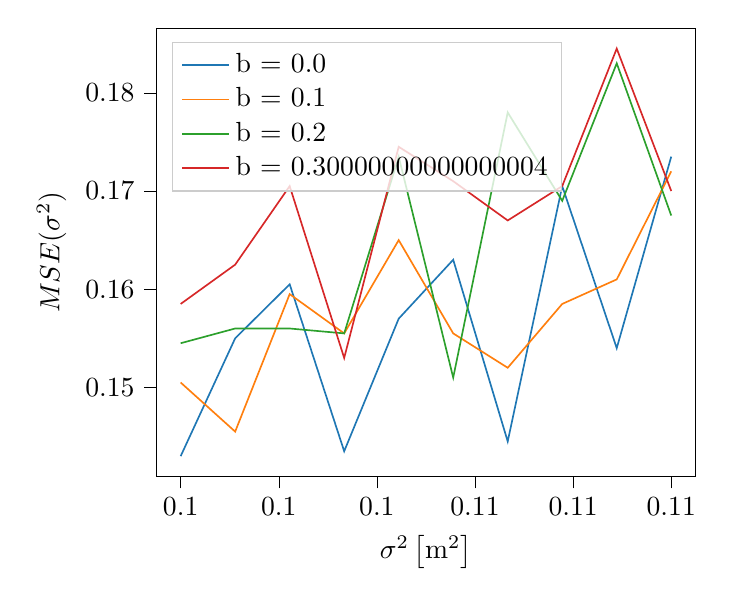
\begin{tikzpicture}

\definecolor{color0}{rgb}{0.12156862745098,0.466666666666667,0.705882352941177}
\definecolor{color1}{rgb}{1,0.498039215686275,0.0549019607843137}
\definecolor{color2}{rgb}{0.172549019607843,0.627450980392157,0.172549019607843}
\definecolor{color3}{rgb}{0.83921568627451,0.152941176470588,0.156862745098039}

\begin{axis}[
legend cell align={left},
legend style={
  fill opacity=0.8,
  draw opacity=1,
  text opacity=1,
  at={(0.03,0.97)},
  anchor=north west,
  draw=white!80!black
},
tick align=outside,
tick pos=left,
x grid style={white!69.0196078431373!black},
xlabel={$\sigma^2 \left[ \si{m}^2 \right]$},
xmin=0.0995, xmax=0.1105,
xtick style={color=black},
y grid style={white!69.0196078431373!black},
ylabel={$MSE(\sigma^2)$},
ymin=0.140925, ymax=0.186575,
ytick style={color=black}
]
\addplot [semithick, color0]
table {%
0.1 0.143
0.101111111111111 0.155
0.102222222222222 0.1605
0.103333333333333 0.1435
0.104444444444444 0.157
0.105555555555556 0.163
0.106666666666667 0.1445
0.107777777777778 0.1705
0.108888888888889 0.154
0.11 0.1735
};
\addlegendentry{b = 0.0}
\addplot [semithick, color1]
table {%
0.1 0.1505
0.101111111111111 0.1455
0.102222222222222 0.1595
0.103333333333333 0.1555
0.104444444444444 0.165
0.105555555555556 0.1555
0.106666666666667 0.152
0.107777777777778 0.1585
0.108888888888889 0.161
0.11 0.172
};
\addlegendentry{b = 0.1}
\addplot [semithick, color2]
table {%
0.1 0.1545
0.101111111111111 0.156
0.102222222222222 0.156
0.103333333333333 0.1555
0.104444444444444 0.1735
0.105555555555556 0.151
0.106666666666667 0.178
0.107777777777778 0.169
0.108888888888889 0.183
0.11 0.1675
};
\addlegendentry{b = 0.2}
\addplot [semithick, color3]
table {%
0.1 0.1585
0.101111111111111 0.1625
0.102222222222222 0.1705
0.103333333333333 0.153
0.104444444444444 0.1745
0.105555555555556 0.171
0.106666666666667 0.167
0.107777777777778 0.1705
0.108888888888889 0.1845
0.11 0.17
};
\addlegendentry{b = 0.30000000000000004}
\end{axis}

\end{tikzpicture}

\end{document}